% Template for ICIP-2018 paper; to be used with:
%          spconf.sty  - ICASSP/ICIP LaTeX style file, and
%          IEEEbib.bst - IEEE bibliography style file.
% --------------------------------------------------------------------------
\documentclass{article}
\usepackage{spconf,amsmath,graphicx}

\graphicspath{ {images/} }

% Example definitions.
% --------------------
\def\x{{\mathbf x}}
\def\L{{\cal L}}

% Title.
% ------
\title{Fine Tuning The Rotating Skip List}
%
% Single address.
% ---------------
\name{Itamar Talmon, Tal Shoef}
\address{Tel Aviv University}

\begin{document}
%\ninept
%
\maketitle
%
\begin{abstract}
Skip list \cite{C3} is a linked-list-based structure that became an increasingly popular concurrent alternative to search trees due to its logerithmic complexity and local balancing operation. The Rotating skip list \cite{C1} is the fastest concurrent skip list to date. In this paper, we investigate, and try to improve upon, the different heuristics used in the Rotating skip list data structure.
\end{abstract}
%
\section{Introduction}
\label{sec:intro}

\subsection{Concurrent Skip Lists}
\label{ssec:csl}
Skip list is a mashu mashu

\subsection{Our Contribution}
\label{ssec:oc}

We examined and extended the following heuristics:

\begin{itemize}
	\item Level Hight Heuristics
	\item Level Delete Heuristics 
	\item Deletion Help Heuristics 
	\item Background Thread Sleeping Heuristics 
\end{itemize}
\\
Detailed descriptions of the changes made, in addition to the evaluations, are included in the prociding sections of the paper.

\subsection{Code Location}
\label{ssec:cl}
The complete code, including the compiled data strucures and the evaluation script, could be find at \\\texttt{github.com/itamartalmon/synchrobench}.

\section{LEVEL HIGHT HEURISTICS}
\label{sec:lhh}

The Maximum Level of the data structure , BLABLABLA

\subsection{Fixed Max Level}
\label{ssec:fml}

Fixing the Max level is commonly use, blablblal

As can be seen on figure BLABLALB, ads
bla bla bla bla bla bla
bla bla bla bla bla 
bla bla bla bla bla bla
bla bla bla bla bla 
bla bla bla bla bla bla
bla bla bla bla bla 
bla bla bla bla bla bla
bla bla bla bla bla bla
bla bla bla bla bla 
bla bla bla bla bla bla
bla bla bla bla bla 
bla bla bla bla bla bla
bla bla bla bla bla 
bla bla bla bla bla bla
bla bla bla bla bla bla
bla bla bla bla bla 
bla bla bla bla bla bla
bla bla bla bla bla 
bla bla bla bla bla bla
bla bla bla bla bla 
bla bla bla bla bla bla

\subsection{Dynamic Max Level}
\label{ssec:dml}

Dynamic Max level is more blablblal

\subsubsection{Evaluation}
\label{sssec:ml-evl}

As can be seen on figure bla bla bla bla bla 
bla bla bla bla bla bla
bla bla bla bla bla 
bla bla bla bla bla bla
bla bla bla bla bla 
bla bla bla bla bla bla
bla bla bla bla bla 
bla bla bla bla bla bla

\begin{figure}
	\caption{Max Level Heuristics Performence}
	\centering
	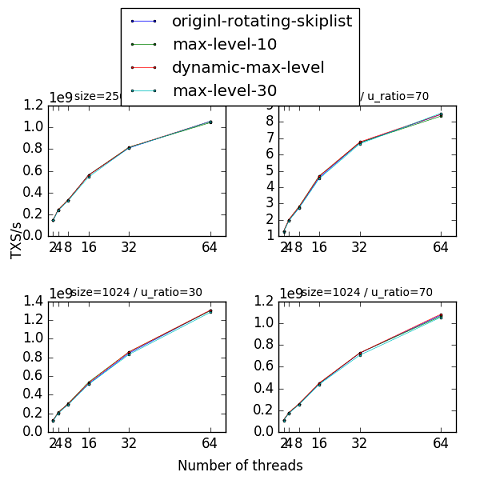
\includegraphics[width=0.4\textwidth]{max-level_plot}
\end{figure}

bli bla blu

\section{ROTAION DELETION HEURISTICS}
\label{sec:rdh}

When deleting blablabae , BLABLABLA

\subsection{Tall-Deletions-Size Rate}
\label{ssec:tds}

In the original paper use, blablblal

\subsubsection{Evaluation}
\label{sssec:tds-evl}

As can be seen on figure BLABLALB, ads
bla bla bla bla bla bla
bla bla bla bla bla 
bla bla bla bla bla bla
bla bla bla bla bla 
bla bla bla bla bla bla
bla bla bla bla bla 
bla bla bla bla bla bla
bla bla bla bla bla bla
bla bla bla bla bla 
bla bla bla bla bla bla
bla bla bla bla bla 
bla bla bla bla bla bla
bla bla bla bla bla 
bla bla bla bla bla bla

\begin{figure}
	\caption{Tall Delelted By Size Deletion Performence}
	\centering
	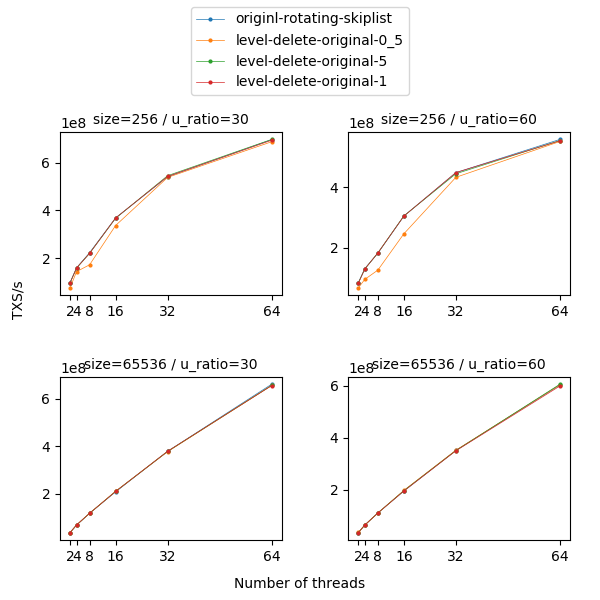
\includegraphics[width=0.4\textwidth]{level-delete-original_plot}
\end{figure}

\subsection{Relative Level Size}
\label{ssec:rls}

Dynamic Max level is more blablblal

\subsubsection{Evaluation}
\label{sssec:rls-evl}

As can be seen on figure BLABLALB, ads
bla bla bla bla bla bla
bla bla bla bla bla 
bla bla bla bla bla bla
bla bla bla bla bla 
bla bla bla bla bla bla
bla bla bla bla bla 
bla bla bla bla bla bla

\begin{figure}
	\caption{Levels Ratio Deletion Performence}
	\centering
	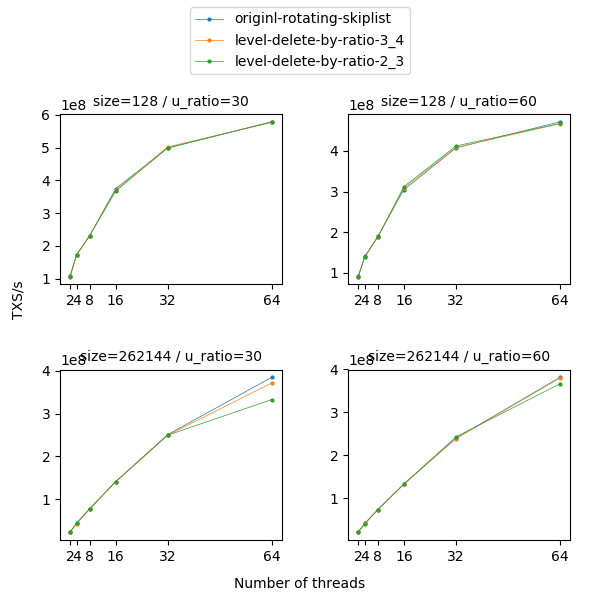
\includegraphics[width=0.4\textwidth]{level-delete-by-ratio_plot}
\end{figure}


\section{DELETION HELP HEURISTICS}
\label{sec:dhh}

\subsection{Thread-Num-Size Rate}
\label{ssec:tns}

Dynamic Max level is more blablblal

\subsubsection{Evaluation}
\label{sssec:tns-evl}

As can be seen on figure BLABLALB, ads
bla bla bla bla bla bla
bla bla bla bla bla 
bla bla bla bla bla bla
bla bla bla bla bla 
bla bla bla bla bla bla
bla bla bla bla bla 
bla bla bla bla bla bla

\begin{figure}
	\caption{Help-Remove Performence}
	\centering
	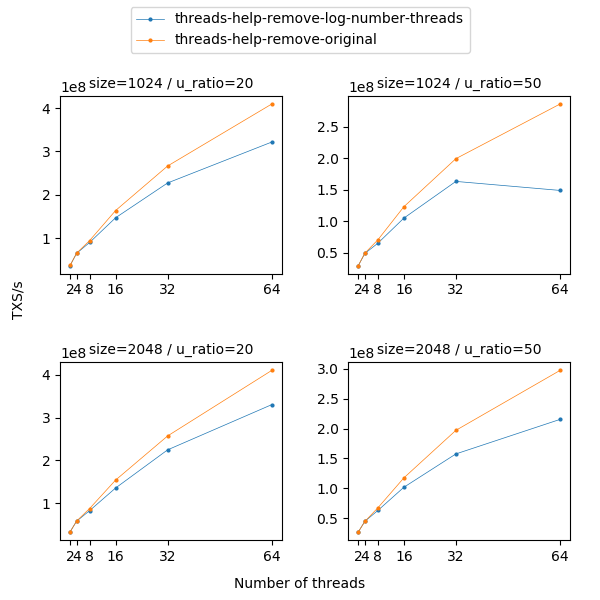
\includegraphics[width=0.4\textwidth]{help-remove_plot}
\end{figure}

\section{BACKGROUND THREAD SLEEP HEURISTICS}
\label{sec:bts}

The background blablabae , BLABLABLA

\subsection{Thread-Num Rate}
\label{ssec:dsrs}

In the original paper use, blablblal

\subsubsection{Evaluation}
\label{sssec:dsrs-evl}

As can be seen on figure BLABLALB, ads

\begin{figure}
	\caption{Background Sleep Time Performence}
	\centering
	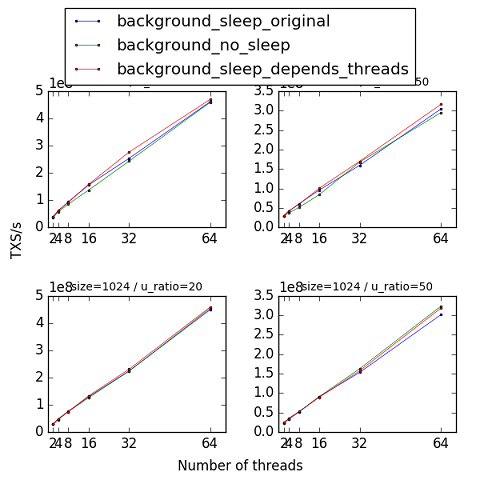
\includegraphics[width=0.4\textwidth]{sleep_plot}
\end{figure}


\section{Experimental Settings}
\label{sec:exp}

In this section we describe the multicore machines and the benchmarks used in our experiments as well as the 7 data structure algorithms we compare our rotating skip list against.
Multicore machines. We used two different multicore machines to validate our results, one with 2 8-way Intel Xeon E5-2450 processors with hyperthreading... BLABLA


\section{Future Research}
\label{sec:foot}

BLIA BALIDSA ADBLADS


% To start a new column (but not a new page) and help balance the last-page
% column length use \vfill\pagebreak.
% -------------------------------------------------------------------------
%\vfill
%\pagebreak


% References should be produced using the bibtex program from suitable
% BiBTeX files (here: strings, refs, manuals). The IEEEbib.bst bibliography
% style file from IEEE produces unsorted bibliography list.
% -------------------------------------------------------------------------
\bibliographystyle{IEEEbib}
\bibliography{refs}

\end{document}
